\chapter{システムの設計・実装}
\label{chap:implementation}

本章では、\ref{chap:network-transmission}章で述べた、映像制作現場におけるIP伝送装置について評価するため、4K映像を非圧縮でIPで伝送するシステムであるNG-HDMI-TSをハードウェアで実装したことについて実装の解説をする。

\section{実装の概要}

IP伝送装置は、Xilinx KC705 評価ボード\cite{xilinx-kc705}、HDMIインターフェースカードであるTED HDMI 2.0 FMCカード\cite{ted-hdmi4k}を使用した。
本実装の構成を図\ref{fig:fpga-implement-flow}に示す。

\begin{figure}[htbp]
  \begin{center}
    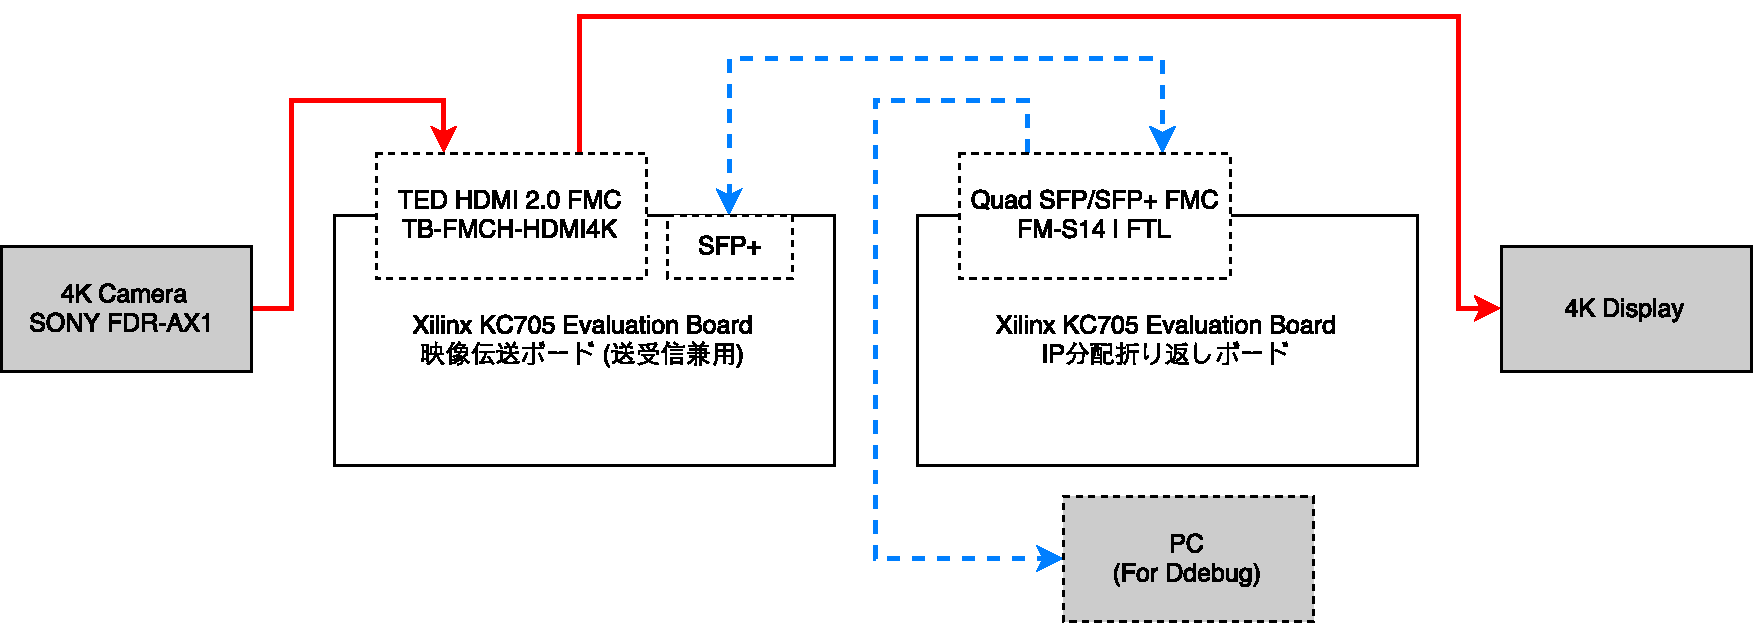
\includegraphics[bb=0 0 841 299,width=15.5cm]{img/fpga-implement-flow.pdf}
  \end{center}
  \caption{ハードウェアによる実装の構成}
  \label{fig:fpga-implement-flow}
\end{figure}

\begin{figure}[htbp]
  \begin{center}
    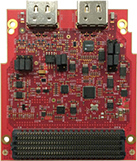
\includegraphics[bb=0 0 137 161,width=4cm]{img/ted-4k-fmc-card.jpg}
  \end{center}
  \caption{TED HDMI 2.0 FMCカード (TB-FMCH-HDMI4K)}
  \label{fig:ted-4k-fmc-card}
\end{figure}

% \begin{table}[htbp]
%   \caption{ハードウェアによる実装を行ったPCの構成}
%   \label{tb:software-specification}
%   \begin{center}
%   \begin{tabular}{c||c}
%     \hline
%     ソフトウェア  & Vivado 2016.2 \\\hline
%   \end{tabular}\end{center}
% \end{table}

今回の構成では、IP伝送装置とは別に1台のXilinx KC705 評価ボード、Quad SFP/SFP+カードを用いて、送信したIPパケットを折り返しする装置を使用した。
IPパケットを折り返しする装置について、IP伝送装置と直接の関係はないため、ここでの解説は割愛する。

本実装では、論理合成ツールとしてXilinx Vivado 2016.2を使用した。また、開発言語としてVerilog HDLを使用した。

\section{FPGAの回路設計}

本実装は、Xilinxが提供しているKintex-7シリーズ向けのHDMI 2.0のリファレンス実装であるxapp1287\cite{xilinx-xapp1287}をベースとている。
Xilinxの提供するIPである10 Gigabit Ethernet Subsystem\cite{xilinx-pg157}、Video PHY Controller\cite{xilinx-pg230}、HDMI 1.4/2.0 Transmitter Subsystem\cite{xilinx-pg235}、及び、HDMI 1.4/2.0 Receiver Subsystem\cite{xilinx-pg236}、FIFO Generator\cite{xilinx-pg057}が使用されている。
本研究のために、新たに実装をした箇所は、これらのIPに対してデータを受け渡しするモジュールとなる。
FPGAの回路全体のブロックダイアグラムを図\label{fig:fpga-whole-diagram}に示す。

\begin{figure}[htbp]
  \begin{center}
    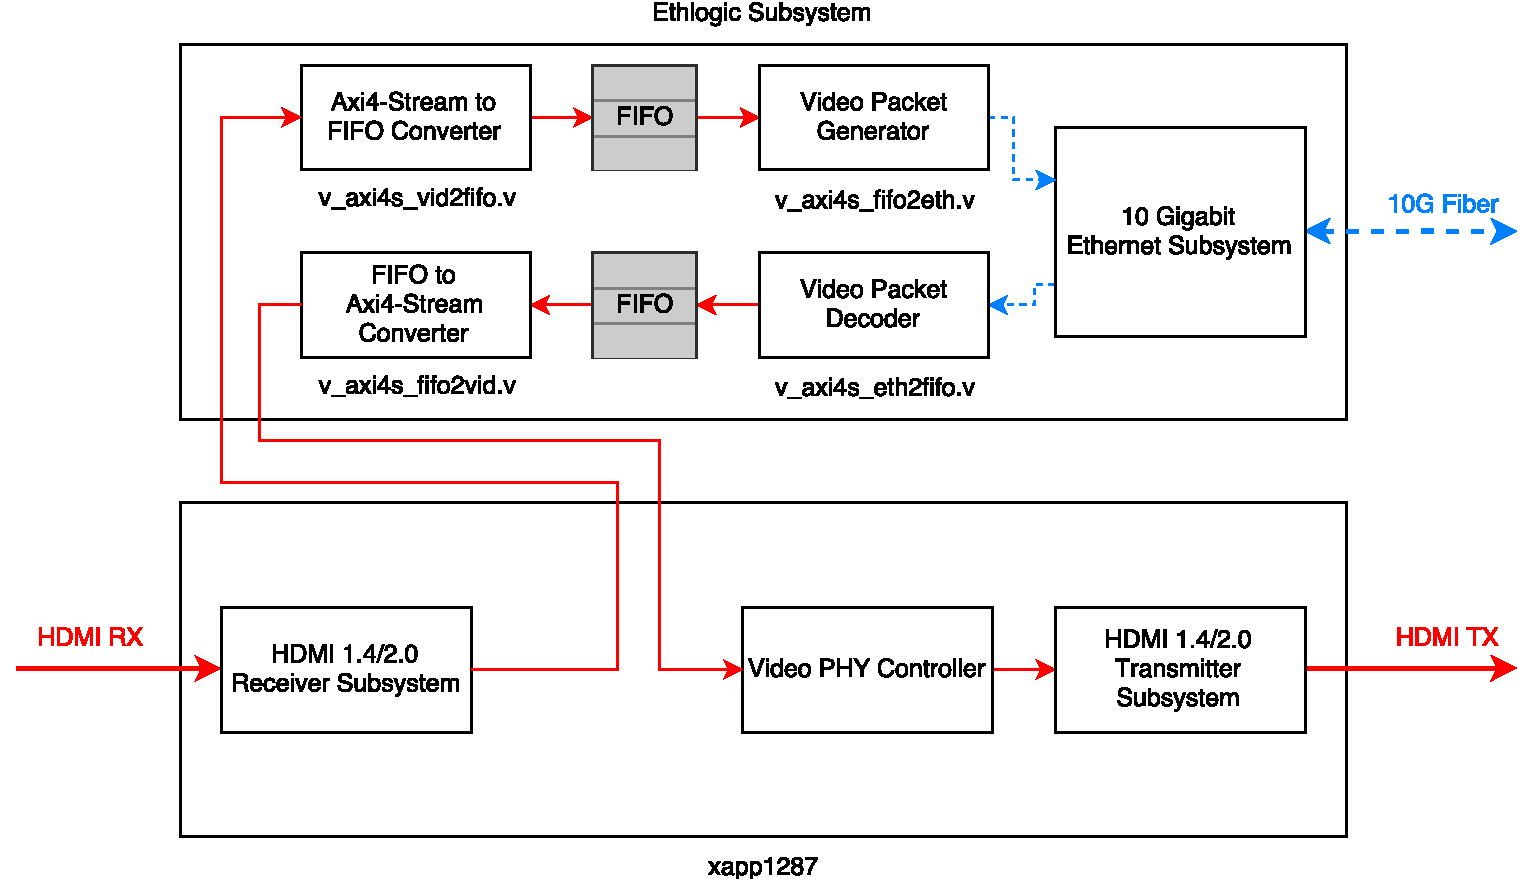
\includegraphics[bb=0 0 452 229,width=15.5cm]{img/fpga-whole-diagram.pdf}
  \end{center}
  \caption{FPGA回路全体のブロックダイアグラム(図は後ほど書く)}
  \label{fig:fpga-whole-diagram}
\end{figure}

受信側と送信側で、10 Gigabit Ethernet SubsystemとVideo Processing Subsystem間の受け渡しを行うため、表\ref{tb:fpga-implement-modules}に示す4つのモジュールを実装した。

\begin{table}[htbp]
  \caption{10 Gigabit Ethernet Subsystem、及び、Video Processing Subsystemの接続のために実装したモジュール}
  \label{tb:fpga-implement-modules}
  \begin{center}
  \begin{tabular}{c|p{12cm}}
    \hline
    Name               & Description \\\hline\hline
    v\_axi4s\_eth2fifo.v & Ethernet Subsystemのクロックで、Ethernet Subsystemから送られてきた映像データをFIFOに書き込むモジュール \\\hline
    v\_axi4s\_fifo2eth.v & Ethernet Subsystemのクロックで、FIFOから読み込んだの映像データをEthernet Subsystemに送るモジュール \\\hline
    v\_axi4s\_vid2fifo.v & Video Processing Subsystemのクロックで、Video Processing Subsystemから送られてきた映像データをFIFOに書き込むモジュール \\\hline
    v\_axi4s\_fifo2vid.v & Video Processing Subsystemのクロックで、FIFOから読み込んだの映像データをVideo Processing Subsystemに送るモジュール \\\hline
  \end{tabular}\end{center}
\end{table}

10 Gigabit Ethernet Subsystemの基準クロックは64bit幅の設定で156.25MHzとなり、Video Processing Subsystemの基準クロックは300MHzとなる。
互いの基準クロックが異なるため、データをそのまま受け渡しすることはできない。

この問題を解決するため、読み書きで独立したクロックに対応したIndependent Clocking FIFOをFIFO Generatorで作成する。
今回のIP伝送装置の送信側で用いた、FIFOのモジュールを図\ref{fig:fpga-independent-clocking-fifo}に示す。

\begin{figure}[htbp]
  \begin{center}
    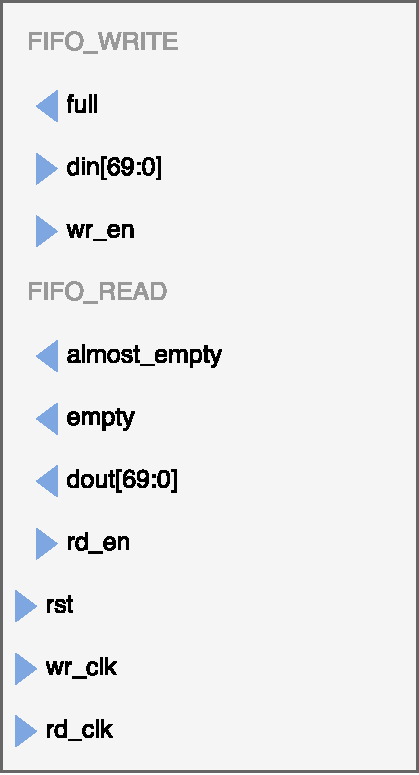
\includegraphics[bb=0 0 201 371,width=4cm]{img/fpga-independent-clocking-fifo.pdf}
  \end{center}
  \caption{Independent Clocking FIFO}
  \label{fig:fpga-independent-clocking-fifo}
\end{figure}

\newpage
読み書きで独立したクロックの他に、入出力のデータ幅が異なっており、入力のデータ幅は35bit、出力のデータ幅は倍の70bitとなっている。理由は後述する。
Video Processing Subsystemは300MHzで35bitのデータを書き込み、10 Gigabit Ethernet Subsystemは156.25MHzのデータを読み込む。
10 Gigabit Ethernet Subsystemのクロックが早いため、FIFOがフル状態になることはない。
また、almost\_emptyフラグを使用しており、emptyになる1クロック前に知ることが可能である。

送信側のモジュールの接続を図\ref{fig:fpga-video-ethernet-diagram}に示す。

\begin{figure}[htbp]
  \begin{center}
    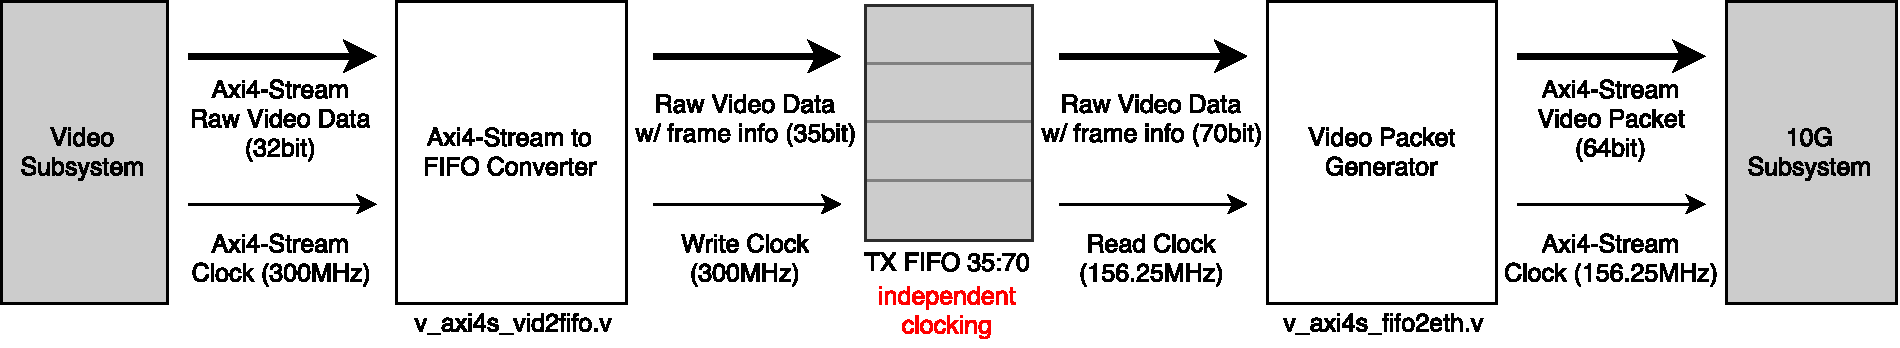
\includegraphics[bb=0 0 911 166,width=15.5cm]{img/fpga-video-ethernet-diagram.pdf}
  \end{center}
  \caption{Video Stream to Ethernet Packet Subsystem Diagram}
  \label{fig:fpga-video-ethernet-diagram}
\end{figure}

受信側のモジュールの接続を図\ref{fig:fpga-ethernet-video-diagram}に示す。

\begin{figure}[htbp]
  \begin{center}
    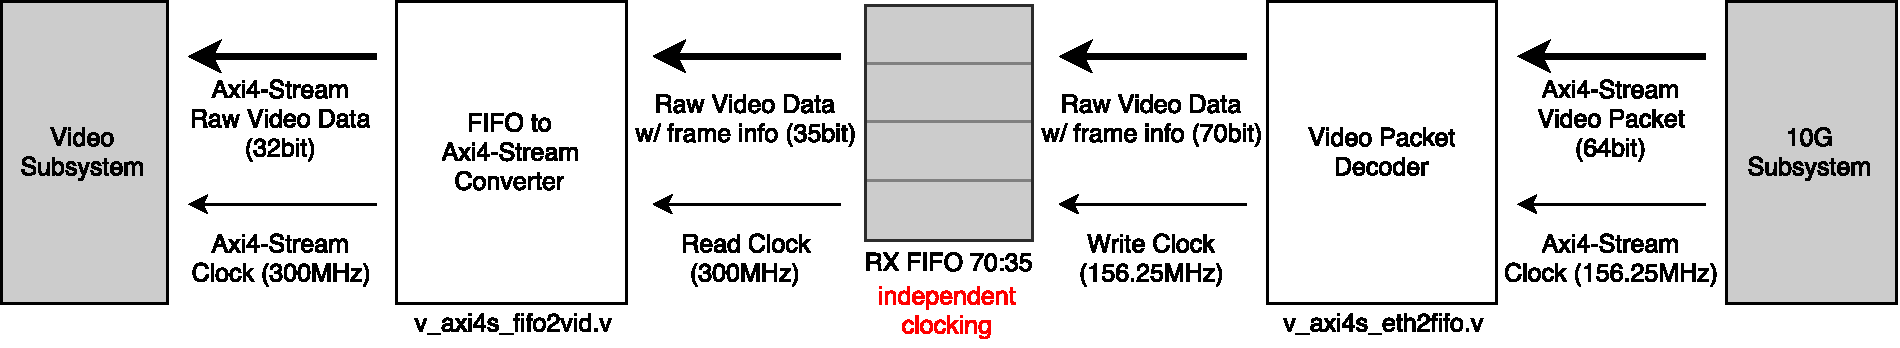
\includegraphics[bb=0 0 911 166,width=15.5cm]{img/fpga-ethernet-video-diagram.pdf}
  \end{center}
  \caption{Ethernet Packet to Video Stream Subsystem Diagram}
  \label{fig:fpga-ethernet-video-diagram}
\end{figure}

Video Processing Subsystemが出力するAxi4-Streamのtdataは映像データを表し、有効データ幅は32bitである。
また、表\ref{tb:fpga-axi4-stream}に示すとおり、tlastがラインの終了、tuserがフレームの開始を表す。
FIFOに映像データだけを書き込んだ場合、ラインの終了、フレームの開始のタイミングが失われることとなる。
この問題を解決するため、FIFOにはAxi4-Streamのtdataの他に、tlast、tuser、tvalidも書き込む。

\begin{table}[htbp]
  \caption{Video Processing SubsystemのAxi4-Streamインターフェース}
  \label{tb:fpga-axi4-stream}
  \begin{center}
  \begin{tabular}{l|c|l}
    \hline
    Name   & Width     & Description \\\hline\hline
    tdata  & 3*BPC\footnote{Max Bits Per Component}*PPC\footnote{Pixels Per Clock} & Data \\\hline
    tlast  & 1         & End of line \\\hline
    tready & 1         & Ready \\\hline
    tuser  & 1         & Start of frame \\\hline
    tvalid & 1         & Valid \\\hline
  \end{tabular}\end{center}
\end{table}

% どちらもAxi4-Stream規格での通信となるが、

% 表\ref{tb:pg236-vout-axi4-stream}
% 表\ref{tb:pg235-vin-axi4-stream}

% Axi4-Stream、tuser
% 図\ref{fig:fpga-video-ethernet-diagram}
% 図\ref{fig:fpga-ethernet-video-diagram}

% Xilinxの 10 Gigabit Ethernet Subsystem、及び、Video Processing Subsystem
% これを解決するため、Xilinxの 10 Gigabit Ethernet Subsystem、及び、Video Processing Subsystem


% また、

% 10 Gigabit Ethernet Subsystemの挙動に空いては、Xilinx PG157\cite{xilinx-pg157}を参照されたし。
% \cite{xilinx-pg235}
% \cite{xilinx-pg236}

% \begin{table}[htbp]
%   \caption{HDMI RX SubsystemのAxi4-Streamインターフェース \cite{xilinx-pg236}より抜粋}
%   \label{tb:pg236-vout-axi4-stream}
%   \begin{center}
%   \begin{tabular}{l|c|c|l}
%     \hline
%     Name   & Direction & Width     & Description \\\hline\hline
%     tdata  & Output    & 3*BPC\footnote{Max Bits Per Component}*PPC\footnote{Pixels Per Clock} & Data \\\hline
%     tlast  & Output    & 1         & End of line \\\hline
%     tready & Input     & 1         & Ready \\\hline
%     tuser  & Output    & 1         & Start of frame \\\hline
%     tvalid & Output    & 1         & Valid \\\hline
%   \end{tabular}\end{center}
% \end{table}
%
%
% \begin{table}[htbp]
%   \caption{HDMI TX SubsystemのAxi4-Streamインターフェース \cite{xilinx-pg235}より抜粋}
%   \label{tb:pg235-vin-axi4-stream}
%   \begin{center}
%   \begin{tabular}{l|c|c|l}
%     \hline
%     Name   & Direction & Width     & Description \\\hline\hline
%     tdata  & Input     & 3*BPC*PPC & Data \\\hline
%     tlast  & Input     & 1         & End of line \\\hline
%     tready & Output    & 1         & Ready \\\hline
%     tuser  & Input     & 1         & Start of frame \\\hline
%     tvalid & Input     & 1         & Valid \\\hline
%   \end{tabular}\end{center}
% \end{table}

図\ref{fig:fpga-video-packet}に、本実装で用いたUDPデータの構造を示す。

\begin{figure}[htbp]
  \begin{center}
    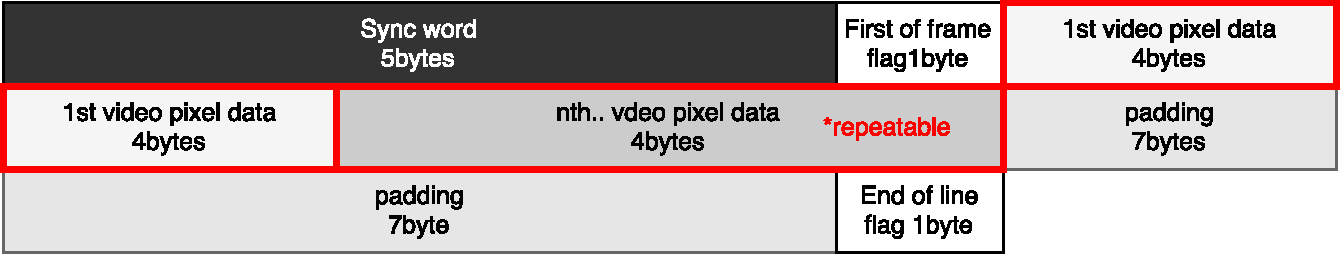
\includegraphics[bb=0 0 643 122,width=15.5cm]{img/fpga-video-packet.pdf}
  \end{center}
  \caption{UDPデータの構造}
  \label{fig:fpga-video-packet}
\end{figure}

UDPデータの映像データより前のヘッダー区間は6byteとなっている。
これは、FPGA内部でEthernetパケットを構築していく際に、データの先頭6byteが丁度64bitの区切り目となるためであり、FPGAで処理する祭に効率が良い。
UDPのパケットはFIFOにデータがある間生成され続けるため、IPパケット上の長さは00としている。映像データによってはジャンボフレームとなる場合もある。

各モジュールで映像データがどのように扱われるかを波形イメージとして、図\ref{fig:fpga-first-pixel-waveform}に示す。

HDMI 1.4/2.0 Receiver Subsystemから出力されるデータは、v\_axi4s\_vid2fifo.vによって、1クロック遅れてFIFOに書き込まれる。
FIFOはある程度のバッファリングが行われるため、一定クロック経過後にemptyが立ち下がり、データが読み取れる状態となる。
v\_axi4s\_fifo2eth.vによって、emptyの立ち下がりの1クロック遅れで、Ethernet、IP、UDPヘッダーの生成を行う。ヘッダーの生成中にも映像データがFIFOにたまり続ける。
ヘッダーの生成がおわる1クロック前にrd\_enを立ち上げ、FIFOのデータを読み取る。UDPデータとして映像データを書き込み、almost\_emptyの立ち下がりでrd\_enを立ち下げる。
% 10 Gigabit Ethernet Subsystem

\begin{figure}[htbp]
  \begin{center}
    % \fbox{
    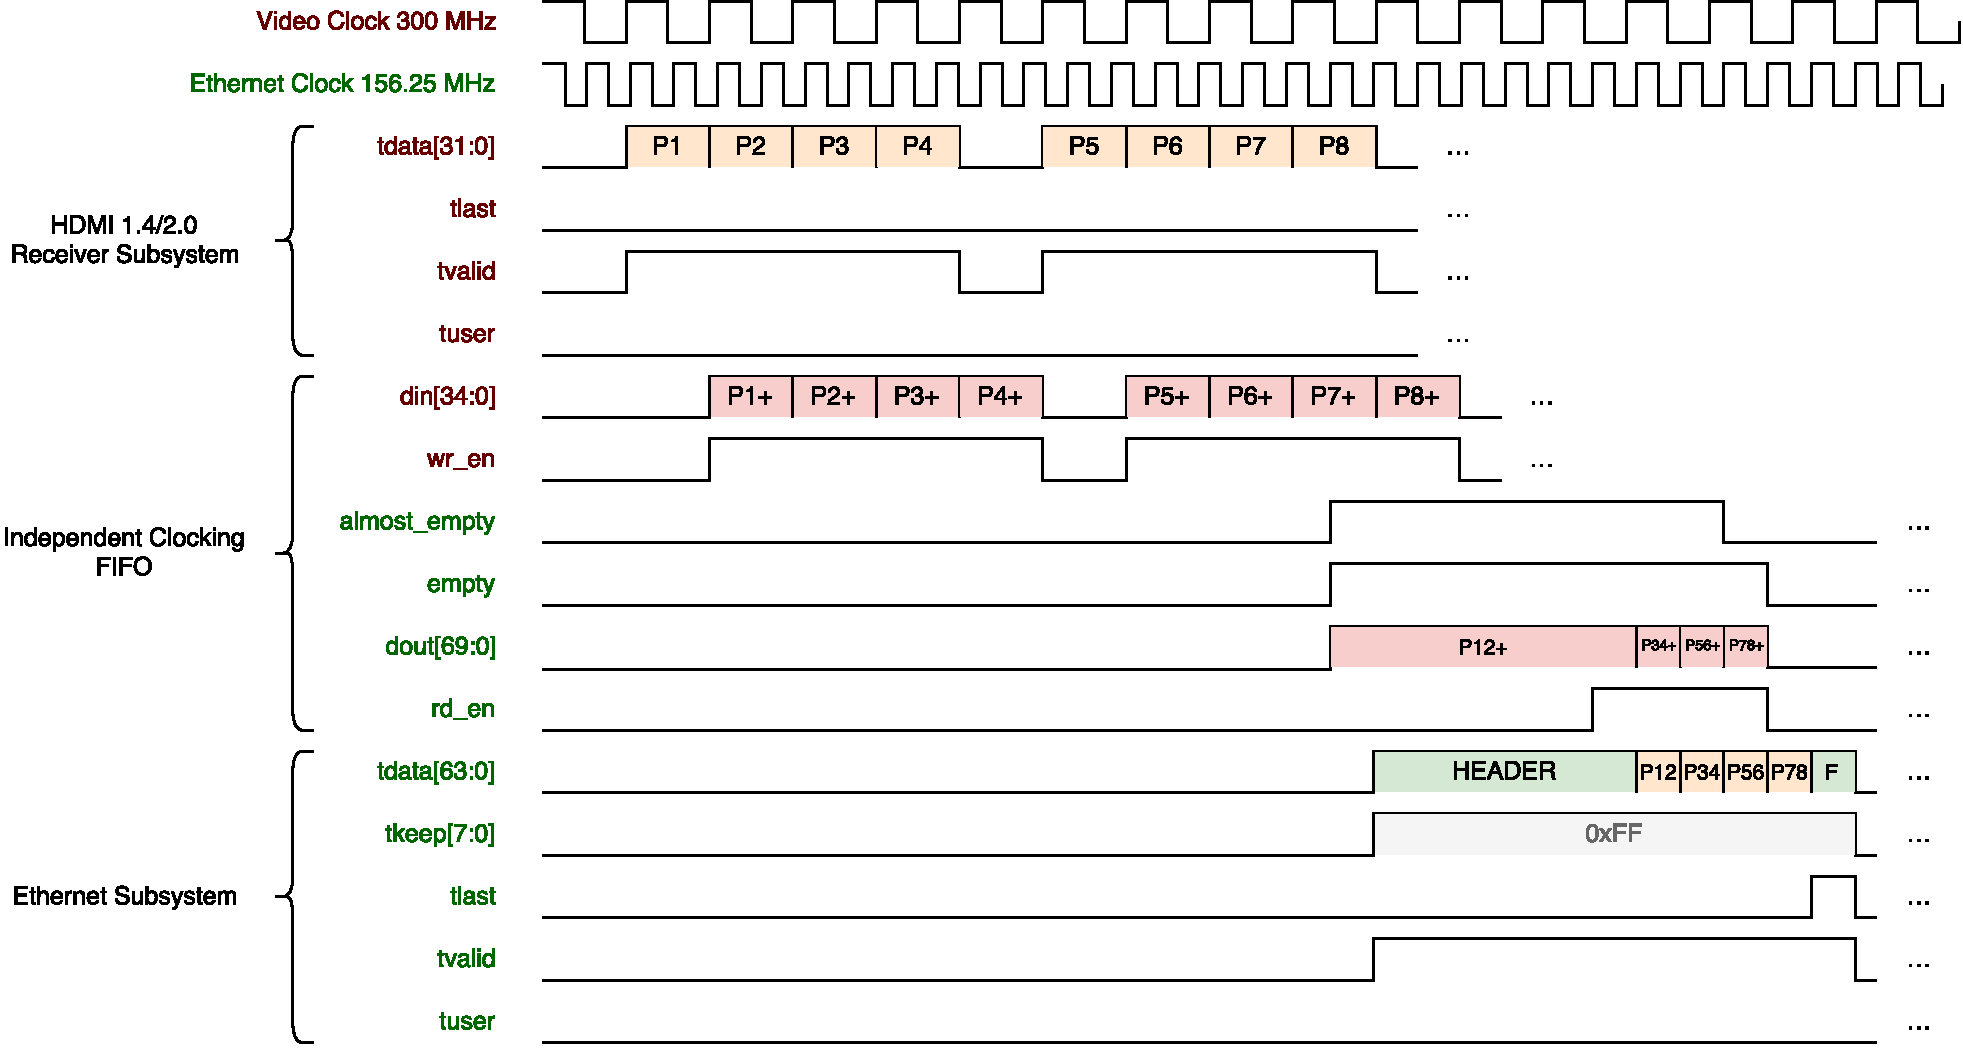
\includegraphics[bb=0 0 942 502,width=22.5cm,angle=270]{img/fpga-first-pixel-waveform.pdf}
    % }
  \end{center}
  \caption{映像データの流れ}
  \label{fig:fpga-first-pixel-waveform}
\end{figure}

% 図\ref{fig:fpga-ila-fifo-to-eth}、
図\ref{fig:fpga-ila-hdmi}では、本実装を稼働させたときのILA(Integrated Logic Analyzer)とよばれる、FPGAの内部信号をモニターするためのツールを使った際に、HDMIの入力と出力を検証した様子である。
前述の通り、almost\_emptyの立ち下がりを合図に、パケットを生成してから映像データを書き込むまでに一定のクロックが経過するため、FIFOへの書き込みがバッファリングされる。
hdmi\_rx\_tvalidが頻繁に立ち上がりと立ち下がりを繰り返しているのに対し、hdmi\_tx\_tvalidはある程度まとまった周期で立ち上がりをしている様子が確認できる。

% \begin{figure}[htbp]
%   \begin{center}
%     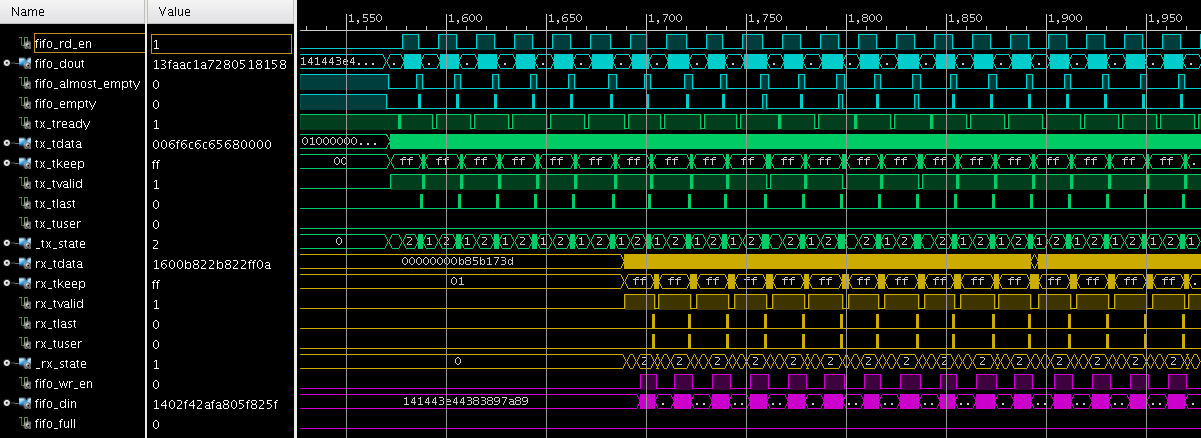
\includegraphics[bb=0 0 1201 438,width=15.5cm]{img/fpga-ila-fifo-to-eth.png}
%   \end{center}
%   \caption{ILAによるIP伝送時のFIFOとEthernet Subsystemのデータのダンプ}
%   \label{fig:fpga-ila-fifo-to-eth}
% \end{figure}

\begin{figure}[htbp]
  \begin{center}
    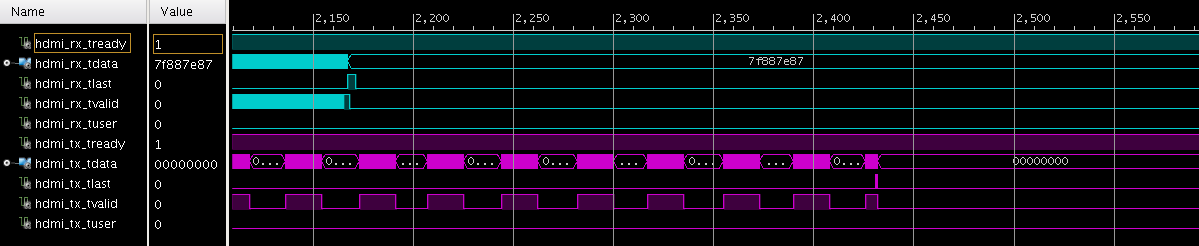
\includegraphics[bb=0 0 1199 246,width=22.5cm,angle=270]{img/fpga-ila-hdmi.png}
  \end{center}
  \caption{ILAによるIP伝送時のHDMI入出力のデータのダンプ}
  \label{fig:fpga-ila-hdmi}
\end{figure}

% \begin{figure}[htbp]
%     \begin{center}
%         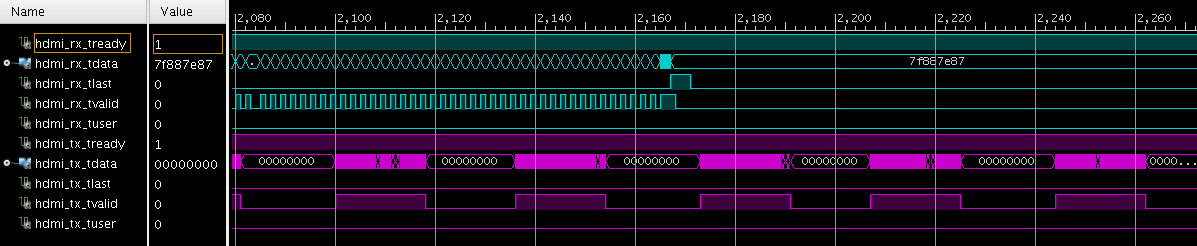
\includegraphics[bb=0 0 1197 246,width=15.5cm]{img/fpga-ila-hdmi-x2.png}
%     \end{center}
%     \caption{図\ref{fig:fpga-ila-hdmi}を拡大した}
%     \label{fig:fpga-ila-hdmi-x2}
% \end{figure}

\begin{table}[htbp]
  \caption{論理合成後のリソース}
  \label{tb:fpga-post-implementation-utilization}
  \begin{center}
  \begin{tabular}{l|r|r|r}
    \hline
    リソース  & 使用    & 全体    & 使用率   \\\hline\hline
    LUT      &  48474 & 203800 & 23.79\% \\\hline
    LUTRAM   &   4696 &  64000 &  7.34\% \\\hline
    FF       &  55768 & 407600 & 13.68\% \\\hline
    BRAM     & 310.50 &    445 & 69.78\% \\\hline
    DSP      &     23 &    840 &  2.74\% \\\hline
    IO       &     40 &    500 &  8.00\% \\\hline
    GT       &      4 &     16 & 25.00\% \\\hline
    BUFG     &     20 &     32 & 62.50\% \\\hline
    MMCM     &      3 &     10 & 30.00\% \\\hline
    PLL      &      1 &     10 & 10.00\% \\\hline
  \end{tabular}\end{center}
\end{table}
